\subsection{Simulation}
Sobald ein möglicher Lösungskandidat anhand der in Abschnitt \ref{sec:kandidatensuche} beschriebenen Suche gefunden
und dessen Initialgeschwindigkeit nach Abschnitt \ref{sec:initialgeschwindigkeit} berechnet wurde,
wird eine Simulation durchgeführt, um die Lösung definitiv zu bestätigen.
Durch das Anwenden verschiedener Anfangsgeschwindigkeiten der weissen Kugel können in diesem Schritt mehrere Situationen evaluiert werden.

Die Simulation wird durch die Definition eines physikalischen Systems wie in Kapitel \ref{kap:physikalisches_system} durchgeführt.
Hierbei gelten die Zuordnungen wie sie nachfolgend beschrieben werden.\\
\textbf{Ereignisse}
\begin{description}
    \item[Energy-Input-Node] Wird modelliert über die Eingabe der Energie der weissen Kugel. Ein spezifischer Node zur
    Modellierung wird nicht implementiert, es wird der Energy-Transfer-Node verwendet, wobei nur der Output-Wert relevant ist.
    \item[Energy-Transfer-Node] Tritt bei der Kollision zwischen zweier Kugeln oder einer Kugel mit der Bande auf.
    \item[No-Energy-Node] Tritt auf, wenn eine Kugel vom dynamischen in den statischen Zustand wechselt (ausrollt). In jedem
    Layer, wo eine Kugel statisch ist, wird sie durch diesen Node modelliert.
    \item[Out-of-System-Node] Sobald eine Kugel mit dem Zielkreis kollidiert, tritt dieses Ereignis auf. Dem System wird die
    Energie entzogen und die Kugel ist nicht mehr verfügbar.
\end{description}

\textbf{Kantenfunktion}
Die Kantenfunktion zwischen den Übergängen innerhalb des Layers bildet der Reibungsverlust der
Kugel über eine bestimmte Zeit oder einen bestimmten Ort.

\textbf{Dynamische/Statische Objekte}
Im Billiard gibt es nur die Kugeln als statische und/oder dynamische Objekte.

\textbf{Konstante Objekte}
Die konstanten Objekte bilden die Banden wie auch die Ziele.

Es wird ungefähr der Pseudoalgorithmus wie in \ref{alg:physikalisches_system} angewendet, optimal auf das Problem \glqq{} Billiard\grqq{}
abgestimmt. Es folgen die physikalischen Berechnungen zur Durchführung der Simulation.


\subsubsection{Reibungsverlust über die Zeit}
Die Geschwindigkeit einer Kugel wird durch die Reibung über die Zeit reduziert. Dazu wird die Formel der gleichförmig
beschleunigten Bewegung verwendet, wobei $\vec{v_0}$, $\vec{a}$ sowie $t$ gegeben sind.
\begin{align}
    \vec{v} = \vec{a} \cdot t + \vec{v_0}
\end{align}

\subsubsection{Elastischer Stoss zweier Kugeln}
Die Kollision zweier Kugeln wird im folgenden als zweidimensionaler elastischer Stoss angesehen. Dabei ist es wichtig,
zwei Komponenten beim Zusammenprall zu betrachten. Dies ist einerseits das Liniensegment $s_z$ zwischen den Mittelpunkten
der Kugeln sowie die orthogonal dazu stehende Gerade $s_t$. Die Kugel, welche Energie mitbringt, übergibt der anderen
Kugel Energie in Richtung von $s_z$. Die übrig gebliebene Energie zeigt in Richtung von $s_t$ \cite{wiki.elastischer_stoss_physik:1}.
In Abbildung \ref{fig:Elastischer Stoss zweier Kugeln} ist ein solcher Stoss dargestellt.
Kugel eins bringt dabei die Geschwindigkeit $\vec{v_1}$ und Kugel zwei die Geschwindigkeit $\vec{v_2}$ mit. Ein Anteil
der Geschwindigkeit von Kugel eins wird der Kugel zwei in Richtung von $s_z$ übergeben. Dasselbe gilt für die
Kugel zwei. Sie übergibt einen Teil ihrer Geschwindigkeit an Kugel eins ebenfalls in Richtung von $s_z$. Die verbleibende
Energie der Kugeln zeigt jeweils in Richtung von $s_t$.
\begin{figure}[h!]
    \begin{center}
        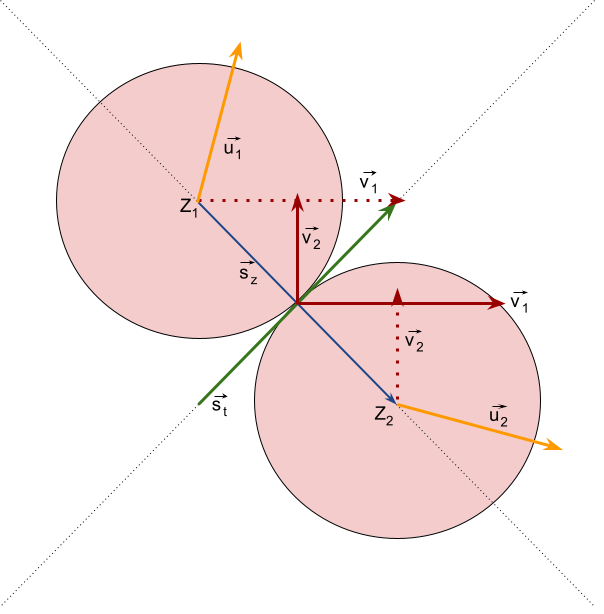
\includegraphics[width=0.4\linewidth]{../common/03_billiard_ai/resources/23_elastischer_stoss.png}
    \end{center}
    \caption{Elastischer Stoss zweier Kugeln}
    \label{fig:Elastischer Stoss zweier Kugeln}
\end{figure}

Die initialen Geschwindigkeiten $\vec{v^i_1}$ und $\vec{v^i_2}$ werden aufgrund eines natürlichen Energieverlusts um eine
Konstante $E_v$, welche in Prozent angegeben wird, reduziert.
\begin{align}
    \vec{v_1} = \vec{v^i_1} \cdot (1 - E_v)\\
    \vec{v_2} = \vec{v^i_2} \cdot (1 - E_v)\\
\end{align}
Um nun die neuen Geschwindigkeiten $\vec{u_1}$ und $\vec{u_2}$ zu berechnen, müssen die initialen Geschwindigkeiten
$\vec{v_1}$ sowie $\vec{v_2}$ auf die Komponenten in Richtung von $s_z$ und $s_t$ aufgeteilt werden.
\begin{align}
    \vec{z} = \vec{Z_2} - \vec{Z_1}\\
    \hat{z} = \frac{\vec{z}}{\norm{\vec{z}}}
\end{align}
Von Interesse ist dabei nur $\hat{z}$. Mittels diesem Vektor kann die Komponente in Richtung von $s_z$ beider Geschwindigkeiten
ausgerechnet werden.
\begin{align}
    \vec{v_{1,z}} = (\vec{v_1} \cdot \hat{z}) \cdot \hat{z}\\
    \vec{v_{2,z}} = (\vec{v_2} \cdot \hat{z}) \cdot \hat{z}
\end{align}
Mittels dieses neuen Vektors in $s_z$ Richtung kann der Vektor in $s_t$ Richtung berechnet werden.
\begin{align}
    \vec{v} = \vec{v_t} + \vec{v_z}\\
    \vec{v_t} = \vec{v} - \vec{v_z}
\end{align}
Daraus folgt für die jeweiligen Kugeln:
\begin{align}
    \vec{v_{1,t}} = \vec{v_1} - \vec{v_{1,z}}\\
    \vec{v_{2,t}} = \vec{v_2} - \vec{v_{2,z}}
\end{align}
Die neuen Geschwindigkeitsvektoren setzen sich wie beschrieben aus den jeweiligen Komponenten zusammen.
Das Resultat lautet wie folgt:
\begin{align}
    \vec{u_1} = \vec{v_{2,z}} + \vec{v_{1,t}}\\
    \vec{u_2} = \vec{v_{1,z}} + \vec{v_{2,t}}
\end{align}
Somit können bei gegebener Kollision zweier Kugeln die Geschwindigkeiten nach der Kollision bestimmt werden.

\subsubsection{Bandenreflektion}
Sofern eine Kugel an eine Bande stösst, so wird diese abgelenkt. In dem hier beschriebenen Modell wird der Drall\cite{wiki.spin:1},
welcher die Bahn einer Kugel nach Kollision mit der Bande ablenken würde, ignoriert.
Das bedeutet, es wird davon ausgegangen, dass der Ausfallswinkel nach der Bandenreflektion gleich dem Eifallswinkel sei.
Dazu kann die folgende Formel\cite{paulbourke.reflected_ray:1} verwendet werden, wobei $I$ der einfallende
und $R$ der ausgehende Weg der Kugel und $N$ der Normalenvektor der Bande sind:
\begin{align}
    R = I - 2 \cdot N \cdot (I \cdot N)
\end{align}

Da bei einer Bandenkollision Energie verloren geht, wird dieses Verhalten mit der Konstanten $E_v$ modelliert.
Diese gibt den Verlust in Prozent an, bezogen auf den minimal berechneten Wert.
\begin{align}
    R = (I - 2 \cdot N \cdot (I \cdot N)) \cdot \frac{1}{1 + E_v}
\end{align}
\subsubsection{Kollisionsprüfung}
Während der Simulation ist es notwendig zu prüfen, welche Kugeln mit welchen kollidieren könnten.
Um zu wissen, ob eine Kugel eine Strecke zurücklegen kann, ohne mit einer anderen Kugel zu kollidieren,
muss für jede andere Kugel geprüft werden, ob diese im Weg liegt. Daher sollte dieser Test effizient sein.
Für den Test wird die zurückzulegende Strecke als Liniensegment zwischen Punkt $A$ und Punkt $B$ und die Position
einer zu testenden Kugel $C$ als Punkt verstanden. Anschliessend wird der Abstand zwischen dem Punkt $C$ und dem
Liniensegment $AB$ geprüft, ob dieser kleiner als der Kugeldurchmesser ist. Sofern dies der Fall ist, liegt die Kugel an
der Position $C$ im Weg und es würde eine Kollision stattfinden, sofern die Ausgangskugel die Strecke $AB$ rollt.
Dies wird für jede Kugel geprüft.


\subsubsection{Ereignis - Energie-Transfer über Kugelkollision}
Dieses Ereignis beschreibt die Kollision mit einer anderen Kugel zum Zeitpunkt $t$.
Bekannt sind dabei die Beschleunigung $\vec{a}$\footnote{Die Beschleunigung $\vec{a}$ ist durch die Herleitung in Kapitel \ref{anhang:herleitung:beschleunigung}
gegeben.}, die Geschwindigkeit $\vec{v}$ und der Ort $\vec{s}$ beider Kugeln.
Diese werden entsprechend indexiert.

Weiterhin sind folgende Abstraktionen bekannt:
\begin{align}
    \vec{\Delta a} = \vec{\Delta a}_1 - \vec{\Delta a}_2\\
    \vec{\Delta v} = \vec{\Delta v}_1 - \vec{\Delta v}_2\\
    \vec{\Delta s} = \vec{\Delta s}_1 - \vec{\Delta s}_2
\end{align}

Es entsteht ein Polynom vierten Grades\footnote{Für Herleitung, siehe Anhang \ref{anhang:herleitung:event:dynamicObjectCollision}}.
Um diese Gleichung zu lösen bedarf es der entsprechenden Lösungsformel \cite{wiki.polynom:1}:
\begin{align}
    ax^4 + bx^3 + cx^2 + dx + e = 0\\
    x_{1,2} = -\frac{b}{4a} - S \pm \frac{1}{2}\sqrt{-4S^2 - 2p + \frac{q}{S}}\\
    x_{3,4} = -\frac{b}{4a} + S \pm \frac{1}{2}\sqrt{-4S^2 - 2p - \frac{q}{S}}\\
    p = \frac{8ac - 3b^2}{8a^2}\\
    q = \frac{b^3 - 4abc + 8a^{2}d}{8a^3}\\
    S = \frac{1}{2}\sqrt{-\frac{2}{3}p + \frac{1}{3a}(Q + \frac{\Delta_0}{Q})}\\
    Q = \sqrt[3]{\frac{\Delta_1 + \sqrt{\Delta_{1}^2 - 4\Delta_{0}^3}}{2}}\\
    \Delta_0 = c^2 - 3bd + 12ae\\
    \Delta_1 = 2c^3 - 9bcd + 27b^{2}e + 27ad^2 - 72ace
\end{align}

Wobei die Koeffizienten folgendermassen lauten:
\begin{align}
    a = \frac{1}{4} \cdot (\vec{\Delta a} \cdot \vec{\Delta a})\\
    b = \vec{\Delta a} \cdot \vec{\Delta v}\\
    c = \vec{\Delta a} \cdot \vec{\Delta s} + \vec{\Delta v} \cdot \vec{\Delta v}\\
    d = 2 \cdot (\vec{\Delta v} \cdot \vec{\Delta s})\\
    e = \vec{\Delta s} \cdot \vec{\Delta s} - D^2
\end{align}

Durch Lösen des Polynoms werden alle Zeitpunkte $x_{1-4} = t_{1-4}$ bestimmt, wobei der relevante Zeitpunkt $t$ der
Erste ist.
\begin{align}
    t = \min{(t_1, t_2, t_3, t_4)}
\end{align}
\newpage
Das Lösen dieses Gleichungssystems erfordert viel Rechenzeit, was die Frage nach Performanceverbesserungen aufwirft.
Diese werden durch Vorbedingungen erzielt, welche welche geprüft werden. Es findet zu Beginn eine Fallunterscheidung
statt. Wenn die zweite Kugel statisch ist, so wird geprüft, ob die Distanz $d$ zwischen der Position $P_2$ der zweiten Kugel
$K_2$ und der halben Geraden $g$ definiert durch die Position $P_1$ der ersten Kugel $K_1$ wie auch deren Geschwindigkeitsvektor
$\vec{v}$ kleiner oder gleich dem Kugeldurchmesser ist. Nur in diesem Fall kann es eine Kollision geben.
Sämtliche Angaben beziehen sich auf die Grafik \ref{fig:kugelkollision_vorbedingung_statisch}.

\begin{figure}[h!]
    \begin{center}
        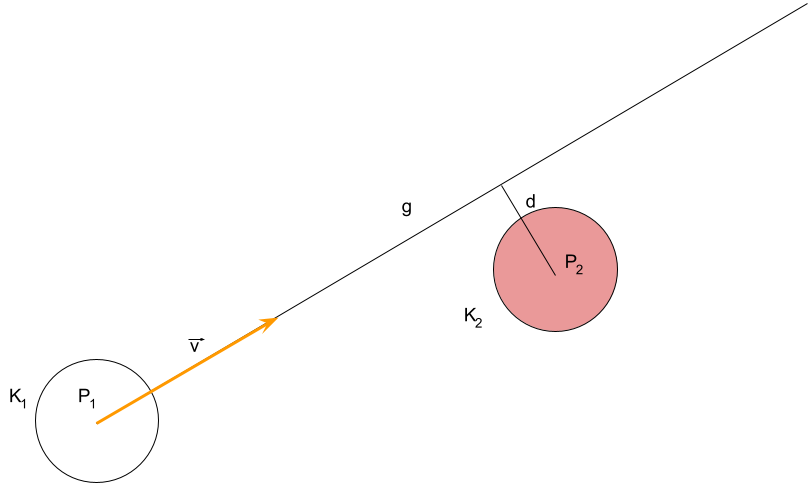
\includegraphics[width=0.4\linewidth]{../common/03_billiard_ai/resources/24_vorbedingung_kugelkollision_statisch.png}
    \end{center}
    \caption{Vorbedingung einer Prüfung auf Kollision zwischen Kugeln bei statischer Beteiligung}
    \label{fig:kugelkollision_vorbedingung_statisch}
\end{figure}

Sobald beide Kugeln dynamisch sind, wird es ein wenig komplizierter. Da beide in Bewegung sind, reicht eine einfache
Prüfung auf die Distanz nicht mehr. Es muss also ein Schnittpunkttest der beiden halben Geraden, definiert durch die
beiden Geschwindigkeitsvektoren, durchgeführt werden. Hierbei ist der Durchmesser der Kugel mitzubeachten, was drei
Spezialfälle eröffnet.
Abbildung \ref{fig:kugelkollision_vorbedingung_dynamisch} zeigt das Vorgehen zur Behandlung des ersten Falls.
Würde nur ein Schnittpunkttest der beiden halben Geraden durchgeführt, so ergäbe diese Situation keine Lösung.
\begin{figure}[h!]
    \begin{center}
        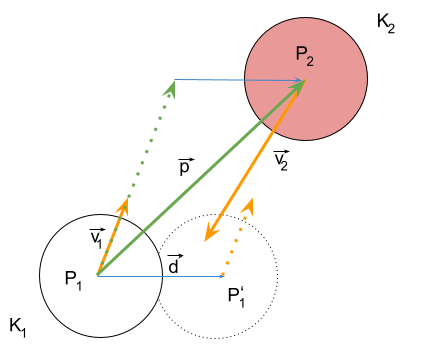
\includegraphics[width=0.4\linewidth]{../common/03_billiard_ai/resources/25_vorbedingung_kugelkollision_dynamisch.png}
    \end{center}
    \caption{Vorbedingung einer Prüfung auf Kollision zwischen dynamischen Kugeln}
    \label{fig:kugelkollision_vorbedingung_dynamisch}
\end{figure}

Daher wird der Vektor $\vec{p}$ zwischen den Positionen $P_1$ und $P_2$ gebildet (grün).
\begin{align}
    \vec{p} = P_2 - P_1
\end{align}
Der erhaltene Vektor wird auf den Geschwindigkeitsvektor $\vec{v_1}$ projiziert (grün gestrichelt).
\begin{align}
    \vec{p'} = (\vec{p} \cdot \hat{v_1}) \cdot \vec{v_1}
\end{align}
Danach wird der Zwischenvektor $\vec{d}$ gebildet (blau).
\begin{align}
    \vec{d} = \vec{p} - \vec{p'}
\end{align}

Die Kugel $K_1$ wird um diesen Vektor verschoben, es resultiert $P^{'}_1$.
\begin{align}
    P^{'}_1 = P_1 + \vec{d}
\end{align}
Von dieser Position aus kann nun ein Schnittpunkttest zwischen den beiden
halben Geraden, durch die Geschwindigkeitsvektoren definiert, durchgeführt werden.

Ein weiterer Spezialfall tritt auf, wenn sich die Kugeln parallel fortbewegen. Da dies ein sehr seltener Fall ist und
wohl kaum auftreten wird, wird die Berechnung zugelassen, wenn der Vektor $\vec{d}$ kleiner oder gleich gross
wie der Durchmesser ist. Die Situation wird in Abbildung \ref{fig:kugelkollision_vorbedingung_dynamisch_parallel} erläutert, die Berechnungen für den Vektor $\vec{d}$
sind äquivalent zum Spezialfall 1.
\begin{figure}[h!]
    \begin{center}
        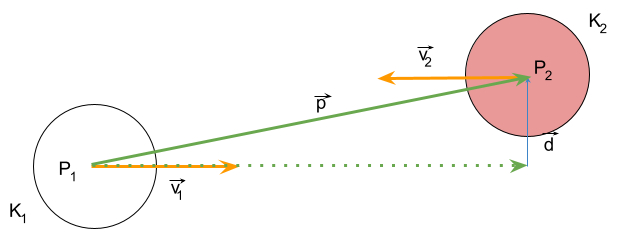
\includegraphics[width=0.4\linewidth]{../common/03_billiard_ai/resources/26_vorbedingung_kugelkollision_dynamisch_parallel.png}
    \end{center}
    \caption{Vorbedingung einer Prüfung auf Kollision zwischen dynamischen parallel velaufenden Kugeln}
    \label{fig:kugelkollision_vorbedingung_dynamisch_parallel}
\end{figure}

Der letzte Spezialfall befasst sich mit der Tatsache, dass ein Schnittpunkttest, so wie er unter Berücksichtigung der
obigen Fälle durchgeführt wird, kein Ergebnis findet, wenn der Schnittpunkt hinter einer der Geraden liegt.
Diese Situation kann in Abbildung \ref{fig:kugelkollision_vorbedingung_dynamisch_hintereinander} entnommen werden.
Es ist ersichtlich, dass der Geschwindigkeitsvektor $\vec{v_1}$ einen grösseren Betrag aufweist als der
Geschwindigkeitsvektor $\vec{v_2}$. Um diesem Umstand Rechnung zu tragen, wird die Startposition der Geraden um den
Durchmesser nach hinten verschoben.
\begin{figure}[h!]
    \begin{center}
        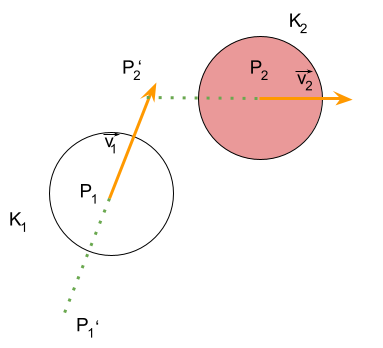
\includegraphics[width=0.4\linewidth]{../common/03_billiard_ai/resources/27_vorbedingung_kugelkollision_dynamisch_hintereinander.png}
    \end{center}
    \caption{Vorbedingung einer Prüfung auf Kollision zwischen dynamischen hintereinander velaufenden Kugeln}
    \label{fig:kugelkollision_vorbedingung_dynamisch_hintereinander}
\end{figure}

\subsubsection{Ereignis - Engergie-Transfer über Bandenkollision}
Dieses Event beschreibt die Kollision mit der Bande. Es soll der Zeitpunkt $t$ der Kollision mit der Bande festgestellt werden.
Der Algorithmus funktioniert so, dass zuerst geprüft wird, ob eine Kollision stattfinden kann.
Dies erfolgt über einen Schnittpunkt-Test zwischen einer Linie und einem Liniensegment.
Eine Bande kann als Liniensegment zwischen dem Startpunkt $R_1$ und $R_2$ betrachtet werden. Diese Punkte müssen demnach bekannt sein.
Weiterhin ist der Geschwindigkeitsvektor $\vec{v}$ und die Position der Kugel $C$ bekannt.
Aufgrund dieser Informationen kann eine Linie definiert werden.

Die Punkte $R_1$ und $R_2$ werden um den Kugelradius zur Tischmitte verschoben,
damit dem Kugelradius Rechnung getragen wird und dieser nicht weiter betrachtet werden muss.
Daraus ergeben sich $R_1'$ und $R_{2'}$\footnote{Für Herleitung, siehe Anhang \ref{anhang:herleitung:event:collisionWithRail}}.

Erster Schritt - Prüfe, ob Kollision möglich:\\
Dazu wird festgestellt, ob ein Schnittpunkt zwischen der Lauflinie der Kugel und dem Liniensegment der
Bande existiert \footnote{Siehe Anhang \ref{anhang:herleitung:event:collisionWithRail}}.
Sofern kein Schnittpunkt vorliegt, können weitere Tests abgebrochen werden, da keine Kollision mit der Bande stattfinden wird.

Zweiter Schritt - Ort der Kollision bestimmen:\\
Betrachte dazu eine der Gleichungen mit zugehörigem $\lambda$:
\begin{align}
    \vec{s(\lambda_1)} = \vec{R_1'} + \lambda_1 \cdot \vec{\Delta R'}\\
    \vec{s(\lambda_2)} = \vec{C} + \lambda_2 \cdot \vec{v}
\end{align}

Dritter Schritt - Zeitpunkt der Kollision bestimmen:\\
Dies kann über die folgenden Gleichungen gelöst werden:
\begin{align}
    \Delta t_1 = \frac{-v + \sqrt{v^2 + 2 \cdot a \cdot \Delta s}}{a}\\
    \Delta t_2 = \frac{-v - \sqrt{v^2 + 2 \cdot a \cdot \Delta s}}{a}
\end{align}
Bevor die Lösung zu $t_1$ und $t_2$ berechnet wird, muss jedoch der Radikand auf folgende Eigenschaft geprüft werden:
\begin{align}
    0 \leq v^2 + 2 \cdot a \cdot \Delta s
\end{align}
Nur in diesem Fall gibt es eine Lösung und somit an dieser Position eine Kollision. Ansonsten hat die Kugel vorher schon
ihre Gesamtenergie verloren und steht still. Es wird das minimum der beiden Zeiten $\Delta t_1$ und $\Delta t_2$ verwendet.

\subsubsection{Ereignis - Totaler Energieverlust}
Dieses Ereignis trifft ein, sobald eine Kugel stillsteht. Der Zeitpunkt wird über die Formel \ref{eq:ereignis:out_of_energy:00}
beschrieben\footnote{Die Herleitung erfolgt in Kapitel \ref{anhang:herleitung:event:outOfEnergy}.
Die Beschleunigung $\vec{a}$ ist durch die Herleitung in Kapitel \ref{anhang:herleitung:beschleunigung}
gegeben.}.

\begin{align}
    t = \max{(\frac{-v_{0,x}}{a_x}, \frac{-v_{0,y}}{a_y})}\label{eq:ereignis:out_of_energy:00}
\end{align}

\subsubsection{Ereignis - Verlassen des Systems}
Der Ereigniszeitpunkt erfolgt über zwei Schritte. Im ersten Schritt wird der Kollisionspunkt der Kugel mit dem
Zielkreis bestimmt. Anhand dieser Information kann die zurückgelegte Distanz der Kugel bestimmt werden.
Es gelten die folgenden Definitionen:\\
$\vec{C} = $ Zielmittelpunkt\\
$\vec{p} = $ Position der Kugel\\
$\hat{v} = $ Normierte Geschwindigkeit der Kugel\\

Die nachfolgende Formel definiert, mit welchem Faktor der Geschwindigkeitsvektor multipliziert werden muss, damit
er die Länge der zurückzulegenden Distanz zum Kollisionsort mit dem Ziel erreicht\footnote{
Für Herleitung, siehe Anhang \ref{anhang:herleitung:event:targetCollision}.}. Zu beachten ist, dass $l$ nur gültig ist,
wenn es grösser als $0$ ist.
\begin{align}
    l_1 = \frac{-(2 \cdot \hat{v} \cdot (\vec{p} - \vec{C})) + \sqrt{4 \cdot (\vec{p} - \vec{C}) \cdot (\vec{p} - \vec{C}) \cdot r^2}}{2}\\
    l_2 = \frac{-(2 \cdot \hat{v} \cdot (\vec{p} - \vec{C})) - \sqrt{4 \cdot (\vec{p} - \vec{C}) \cdot (\vec{p} - \vec{C}) \cdot r^2}}{2}\\
    l = \max{(\min{(l_1, l_2)}, 0)}\\
    \vec{d(l)} = l \cdot \hat{v}
\end{align}

Nachdem die Distanz bestimmt wurde, kann der Kollisionszeitpunkt berechnet werden\footnote{Für Herleitung, siehe Anhang \ref{anhang:herleitung:event:targetCollision}.
Die Beschleunigung $\vec{a}$ ist durch die Herleitung in Kapitel \ref{anhang:herleitung:beschleunigung} gegeben.}.
Zu beachten ist, dass keine Lösung existiert, wenn die Diskriminante kleiner denn $0$ ist. Die Kugel rollt zu langsam und
der Reibungsverlust ist zu gross, als dass sie den Zielkreis erreichen könnte.
\begin{align}
    t_1 = \frac{-\norm{\vec{v}} + \sqrt{\norm{\vec{v}}^2 + 2 \cdot \norm{\vec{a}} \norm{\vec{d(l)}}}}{\norm{\vec{a}}}\\
    t_2 = \frac{-\norm{\vec{v}} - \sqrt{\norm{\vec{v}}^2 + 2 \cdot \norm{\vec{a}} \norm{\vec{d(l)}}}}{\norm{\vec{a}}}\\
    t = \min{(t_1, t_2)}
\end{align}